%%\documentclass[male, authorStatement, indexNumber, fileVersion, keywords, thanks]{lib/uekthesis}
\documentclass[indexNumber, fileVersion]{lib/uekthesis}
\usepackage{lib/uekthesis}



%##############################################################################
% Zmienne Globalne !!! - ważne by kodowanie UTF-8 było wstawione przed nimi
%
% To zmiennne do modyfikacji przez użytkownika
%
\globalFullAuthor{Jan Kowalski}                     % Pełna nazwa autora pracy
\globalShortAuthor{J.\ Kowalski}                     % Autor - zwięzła forma wydruku
\globalFullTitle{Przygotowanie pracy dyplomowej \\[2mm]
przy użyciu oprogramowania LaTeX}  % Pełny tytuł pracy
\globalShortTitle{Praca dyplomowa w systemie LaTeX}       % Krótki, zwięzły tytuł pracy
\globalFullUniversity{Uniwersytet Ekonomiczny w Krakowie} % Pełna nazwa uniwersytetu
\globalShortUniversity{UEK}                           % Skrócona nazwa uniwersytetu
\globalDepartment{Instytut Zarządzania}                % Wydział
\globalDegreeprogramme{Informatyka Stosowana\\Inżynieria oprogramowania}         % Kierunek i specjalność studiów
\globalThesisType{Praca dyplomowa}                    % Typ pracy dyplomowej
\globalUnderTheSupervisonOf{Pod kierunkiem}
\globalSupervisor{prof. dr hab. Jana Iksińskiego}  % Promotor
\globalFileVersion{0.1.0}   % wersja pliku
\globalIndexNumber{123456}  % nr indeksu studenta
\globalCity{Kraków}         % miasto
\globalYear{2019}           % rok powstania pracy
\globalKeywords{nauka, komputery, praca dyplomowa, latex, uczelnia, student} % słowa kluczowe dla pracy

%##############################################################################
% Dołączenie pliku bibliografii zgodnej z Biblatex
\addbibresource{bibliography.bib}

%##############################################################################
% dodatkowe pakiety
%\usepackage{chemfig} % wzory chemiczne

% Lista słów (dzielenia je, lub nie)
\hyphenation{LaTeX latex LaTeXu}

%##############################################################################
% Koniec preambuły i rozpoczęcie treści właściwej dokumentu
\begin{document}
\nocite{*}

\titlepages
\tableofcontents
\clearpage

% Tu umieszczamy rozdziały w porządanej kolejności 
\chapter*{Wstęp}
\label{chap:wstep}
\addcontentsline{toc}{chapter}{Wstęp}
\addtocounter{chapter}{0}
\sectionmark{Wstęp} % changes the head for the current page

Praca dyplomowa (licencjacka, magisterska) to pisemne opracowanie wykonane samodzielnie przez studenta pod kierunkiem promotora, stanowiące sprawozdanie z przeprowadzonych przez autora działań. Zalecana objętość pracy licencjackiej to około 50–70 stron, natomiast pracy magisterskiej 60-80 stron. Temat pracy powinien być powiązany z dziedziną wiedzy reprezentowaną przez uczelnię, a także odnosić się do realizowanego przez studenta kierunku kształcenia.

Niniejszy dokument zawiera podstawowe informacje, które powinny ułatwić studentowi przygotowanie poprawnej pracy, zgodnej z wymogami stawianymi pracom dyplomowym \cite{dirac}. Jednocześnie dokument ten można bezpośrednio wykorzystać przy tworzeniu pracy dyplomowej. Został on podzielony na: wstęp, trzy rozdziały oraz zakończenie, umiejscowione w oddzielnych plikach. Należy zatem zastąpić tekst umieszczony w tych plikach tekstem pracy dyplomowej. Formatowanie dokumentu zostanie dokonane automatycznie, w oparciu o opracowany szablon pracy dyplomowej.

Wstęp pracy dyplomowej powinien zawierać ogólny zarys i tło badanego problemu oraz przesłanki dla podjęcia realizowanego tematu. Ponadto we wstępie należy jasno sformułować cel i zakres pracy, pytania badawcze oraz scharakteryzować krótko sposób realizacji tematu. Należy również przedstawić skrótowo, co będzie przedmiotem poszczególnych rozdziałów pracy. Wstęp powinien liczyć co najmniej 350 słów.
\chapter{Forma pracy}
\label{chap:forma_pracy}



\section{Objaśnienie pojęć}

Zwyczajowo praca dyplomowa posiada formę pisemnego opracowania i składa się z trzech do czerech rozdziałów, wstępu oraz zakończenia co stanowi opis samodzielnie rozwiązanego zadania. Początkowe rozdziały pracy zawierają rozwinięcie (objaśnienie) pojęć występujących w tytule pracy (przegląd literatury) stanowiąc wstęp teoretyczny do własnego „wkładu” dyplomanta w rozpracowanie tematu pracy.



\section{Wkład własny dyplomanta}

Ostatni rozdział pracy stanowi zwykle wkład własny dyplomanta w rozwój nauki, czy też pokazuje umiejętność wykorzystania zdobytej wiedzy autora pracy podczas realizowanych studiów. W zależności od rodzaju pracy dyplomowej (licencjacka, magisterska) może ona posiadać charakter czysto teoretyczny, może stanowić rezultat przeprowadzanych obserwacji, czy też posiadać charakter zawodowy


\subsection{Badania empiryczne}

Badanie empiryczne (ankieta) mająca na celu odpowiedź na pytanie badawcze sformułowane przez dyplomanta. Etapy:

\begin{itemize}
	\item zdefiniowanie pytań (ankiety),
	\item implementacja ankiety (można zrobić to prosto korzystając z formularzy Google),
	\item badania pilotażowe - wstępna weryfikacja zrozumiałości ankiety, czyli przetestowanie ankiety na kilku osobach,
	\item badania właściwe skierowane do docelowej grupy respondentów,
	\item przedstawienie wyników ankiety, 
	\item analiza/dyskusja wyników ankiety, odpowiedź na pytanie badawcze,
	\item wnioski – podsumowanie.
\end{itemize}


\subsection{Analiza przypadku (case study)}

Etapy:

\begin{itemize}
	\item znalezienie „przypadku” do analizy, w którym dzieją się sprawy związane z tematem pracy (może to być firma, urząd, … - jednostka, do której magistrant ma dostęp czy to ze względu na swoją pracę czy też znajomości z osobami tam pracującymi),
	\item  wywiady z pracownikami jednostki (trzeba wcześniej przygotować zestaw interesujących dyplomanta pytań), przeglądanie materiałów jednostki i innych źródeł mających związek z tematem pracy,
	\item  przedstawienie wyników (opis jednostki, opis zagadnień związanych z tematem pracy),
	\item analiza/dyskusja wyników ankiety, odpowiedź na pytanie(a) badawcze,
	\item  wnioski – podsumowanie.
\end{itemize}


\subsection{Aplikacja}

Opis programu, wykonanego przez dyplomanta, który stanowi ilustrację/rozwiązanie problemu przedstawionego w pierwszych rozdziałach pracy.


\subsection{Model (Framework)}

Model teoretyczny opracowany przez dyplomanta, który powstał na bazie przeglądu literatury przedstawionego w początkowych rozdziałach pracy.


\subsection{Krytyczny przegląd literatury}

Systematyczny przegląd literatury mający dać odpowiedź na sformułowane pytanie badawcze. Etapy:

\begin{itemize}
	\item określenie baz bibliograficznych, które będzie się brało się pod uwagę (Web of Science, Scopus, Google scholar, Springer Link, …),
	\item zdefiniowanie słów kluczowych według, których będzie się przeszukiwało bazy danych,
	\item określenie zakresu czasowego przeszukiwań (z jakich lat?) oraz rodzaju źródeł (książki?, artykuły?,…),
	\item przedstawienie wyników wyszukiwań (liczba pozycji pojawiających się jako wyniki wyszukiwań, liczby „odrzuconych” pozycji, liczba pozycji dokładnie analizowanych, jakie zagadnienia były poruszane w jakich publikacjach, …),
	\item analiza/dyskusja wyników ankiety, odpowiedź na pytanie(a) badawcze, wnioski – podsumowanie.
\end{itemize}


\chapter{Redagowanie tekstu}
\label{chap:redagowanie_tekstu}



\section{Tekst zasadniczy pracy}

Praca powinna zostać podzielona na rozdziały oraz podrozdziały. Rozdziały nie powinny być zbyt krótkie, każdy z nich powinien zawierać co najmniej 3500 słów. Tytuły rozdziałów oraz podrozdziałów należy sformatować przy użyciu właściwych stylów (Nagłówek 1, Nagłówek 2, Nagłówek 3), w celu zapewnienia możliwości automatycznego tworzenia spisu treści. Należy zwrócić uwagę, iż po tytułach rozdziałów/podrozdziałów nie stosuje się znaku kropki.

Poszczególne paragrafy pracy (zasadniczy tekst rozdziałów) należy konstruować zgodnie z wymaganą strukturą zaprezentowaną przez Bryson (2014). Paragrafy nie powinny być zbyt krótkie, każdy z nich powinien zawierać co najmniej 5 zdań. Dla sformatowania tekstu zasadniczego pracy należy wykorzystać styl Normalny. Należy również zwrócić uwagę na występujące w dokumencie puste paragrafy (niezawierające tekstu), które należy bezwzględnie usunąć.

W treści pracy dyplomowej należy używać wyłącznie języka formalnego, stosując typowe w takich opracowaniach wyrażenia i zwroty (Zimny, n.d.). Należy również unikać stosowania formy osobowej w tekście pracy. Należytej uwagi wymaga również stosowanie skrótów. Każde pierwsze wystąpienie skrótu w dokumencie powinno zostać uzupełnione pełnym jego objaśnieniem, podanym w nawiasie, np. UEK (Uniwersytet Ekonomiczny w Krakowie). Kolejne użycia skrótu w dokumencie nie wymagają już podawania jego rozwinięcia.



\section{Lista wypunktowana}

W przypadku użycia takiej listy w redagowanym dokumencie należy kierować się poniższymi zasadami:

\begin{itemize}
\item zdanie poprzedzające listę wypunktowaną powinno zostać zakończone znakiem dwukropka,
\item każdy punkt listy powinien rozpoczynać się z małej litery,
\item na końcu każdego punktu listy należy umieścić przecinek, natomiast ostatni punkt powinien zostać zakończony kropką.
\end{itemize}

Należy również zaznaczyć, iż lista wypunktowana nie powinna stanowić zakończenia rozdziału czy podrozdziału pracy.



\section{Lista numerowana}

W przypadku użycia takiej listy w redagowanym dokumencie należy kierować się poniższymi zasadami:

\begin{enumerate}
\item Zdanie poprzedzające listę numerowaną powinno zostać zakończone znakiem dwukropka.
\item Każdy punkt listy numerowanej powinien rozpoczynać się z wielkiej litery.
\item Na końcu każdego punktu listy należy umieścić znak kropki.
\end{enumerate}

Należy również zaznaczyć, iż lista numerowana nie powinna stanowić zakończenia rozdziału czy podrozdziału pracy.





\chapter{Rysunki i tabele}
\label{chap:rysunki_tabele}



\section{Rysunki}

Należy zwrócić szczególną uwagę na redagowanie rysunków (wykresów, zdjęć, schematów, itp.). Każdy rysunek powinien posiadać tytuł, kolejny numer oraz źródło pochodzenia. Do każdego rysunku należy umieścić odniesienie w tekście pracy zawierające jego numer. Pierwsze odwołanie musi wystąpić przed pojawieniem się rysunku w dokumencie, przy czym rysunek nie musi występować bezpośrednio po tym odwołaniu, np.

(...) z danych przedstawionych na rysunku \ref{fig:inflacja} wynika, iż w Polsce zaobserwować można powolny wzrost inflacji począwszy od drugiego półrocza 2017 roku (...)

Stosując odwołania należy bezwzględnie odnosić się do numeru rysunku, nie powinno stosować się sformułowań „powyżej/poniżej”. Bardzo istotna jest również jakość użytych ilustracji. Najlepiej, aby rysunki zostały sporządzone samodzielnie przez autora pracy. Należy unikać umieszczania w pracy kopii rysunków (skanów) o wątpliwej jakości, zaczerpniętych z innych źródeł. Rzutuje to na ostateczną ocenę pracy. Ważne jest również zachowanie spójnej kolorystyki dla wszystkich rysunków wykorzystanych w pracy.

\begin{figure}[ht]
	\centering
	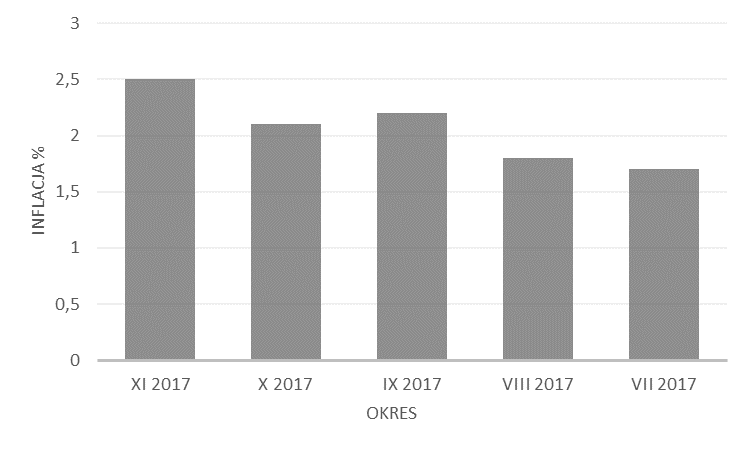
\includegraphics[width=150mm]{images/inflacja.png}
	\captionsource{Inflacja w Polsce.}{opracowanie własne.}
	\label{fig:inflacja}
\end{figure}

Na końcu pracy należy umieścić wykaz (spis) występujących w pracy rysunków uporządkowany wg kolejności ich występowania w dokumencie.



\section{Tabele}

Należy zwrócić szczególną uwagę na redagowanie tabel. Każda tabela powinna posiadać tytuł, kolejny numer oraz źródło pochodzenia danych. Tabelę należy wyśrodkować na stronie dokumentu. Jeśli to możliwe, powinno unikać się dzielenia tabel i umieszczać je w całości na jednej stronie. Do każdej tabeli należy umieścić odniesienie w tekście pracy zawierające jej numer. Pierwsze odwołanie musi wystąpić przed pojawieniem się tabeli w dokumencie, przy czym tabela nie musi występować bezpośrednio po tym odwołaniu, np. na tej samej stronie, np.

(...) z danych przedstawionych w tabeli \ref{tab:inflacja} wynika, iż w Polsce zaobserwować można powolny wzrost inflacji począwszy od drugiego półrocza 2017 roku (...)

\begin{table}[ht]
	\captionsource{Inflacja w Polsce.}{opracowanie własne.}
	\label{tab:inflacja}
	\centering
	\begin{tabular}{ l c }
		\hline
		\textbf{Okres}  &  \textbf{Wartość} \\ \hline
		XI 2017         &  2,5 \\
		X 2017          &  2,1 \\
		IX 2017         &  2,2 \\
		VIII 2017       &  1,8 \\
		VII 2017        &  1,7 \\ \hline
	\end{tabular}
	
\end{table}

 Wszystkie tabele występujące pracy powinny zostać sformatowanie w jednolity sposób i wyśrodkowane. Tytuł tabeli należy umieścić nad tabelą, a do jego formatowania wykorzystać styl Tytuł tabeli. Pod tabelą należy bezwzględnie podać źródło pochodzenia tabeli. Paragraf ten należy sformatować przy użyciu stylu Źródło.


Na końcu pracy należy umieścić wykaz (spis) występujących w pracy tabel uporządkowany wg kolejności ich występowania w dokumencie.



\section{Wzory}

Tu przykłady stosowania wzorów, np.

\begin{equation}
a^x+y \neq a^{x+y}
\end{equation}






\chapter{Literatura naukowa}
\label{chap:literatura_naukowa}



\section{Bazy publikacji naukowych}

Tworząc pracę dyplomową stajemy przed koniecznością zapoznania się szerzej z realizowanym zagadnieniem. Pomocne w tym będą bazy danych publikacji naukowych. Witryna internetowa UEK (\url{https://kangur.uek.krakow.pl/?q=pl/zbiory/bazy-danych})
umożliwia dostęp do międzynarodowych baz danych, w szczególności:

\begin{itemize}
	\item Springer Link (pełne teksty artykułów, czy książek),
	\item Scopus,
	\item Web of Science.
\end{itemize}



\section{Baza Google Scholar}

Jedną z ogólnodostępnych baz jest również Google Scholar. Korzystanie z niej jest niezmiernie proste. Należy:

\begin{itemize}
	
	\item przejść do witryny \url{https://scholar.google.pl},
	
	\item wprowadzić ciąg do wyszukiwania, np. dla uzyskania informacji o publikacjach naukowych, które dotyczą zalet i wad wykorzystania e-learningu należy wpisać:\\
	\textbf{e-learning zalety wady} lub też \textbf{e-learning advantages disadvantages},
	
	\item zawęzić wyniki wyszukiwania (np. do publikacji z ostatnich kilku lat lub ustalić inne kryteria filtrowania),
	
	\item przejrzeć odszukane publikacje; zapoznać się z ich opisem,
	
	\item pobrać wersję elektroniczną publikacji (dla sporej liczby publikacji dostępna jest wersja elektroniczna w formatach PDF, HTML, itp.).
	
\end{itemize}


W przypadku chęci powołania się na odszukaną w bazie publikację należy skorzystać z symbolu znaku cudzysłowu znajdującego się w ostatnim wierszu opisu publikacji. Kliknięcie w ten symbol spowoduje wyświetlenie opisu bibliograficznego publikacji w powszechnie używanych formatach. Należy skopiować opis w formacie BibTex do ... . Następnie można przywołać tę publikację (zacytować ją) w tekście swojej pracy dyplomowej.



\section{Bibliografia}

Bibliografia zawiera spis prac, które zostały wykorzystane w redagowanym dokumencie (do których istnieje cytowanie w tekście dokumentu). Spis prac powinien zostać uporządkowany alfabetycznie. Należy sporządzić go w oparciu o zestaw reguł APA (American Psychological Association), który jest jednym z najczęściej stosowanych w cytowaniu źródeł w naukach społecznych. Dostępne są liczne opracowania dotyczące zasad formatowania APA dla książek, artykułów w czasopismach, źródeł internetowych, dokumentów elektronicznych, itp. (Harasimczuk \& Cieciuch, 2012; APA, 2018; APA Style). Należy zwrócić uwagę na użycie w cytowaniach wyłącznie nazwisk, bez imienia (inicjału imienia) autora.

Dla przywołania pracy wymienionej w bibliografii w tekście redagowanego dokumentu należy również stosować zestaw reguł APA. Nie należy wykorzystywać do tego celu przypisów dolnych . Należy również zwrócić uwagę, aby każda praca wymieniona w bibliografii została przywołana (zacytowana) w tekście redagowanego dokumentu przynajmniej jednokrotnie. W przypadku dosłownego cytowania, należy podać również numer strony, gdzie cytowany tekst występuje, zgodnie ze specyfikacją APA.

Bibliografia, w przypadku pracy dyplomowej, powinna zawierać co najmniej 20 pozycji, z którymi student dokładnie się zapoznał i wykorzystał je w redagowanym dokumencie, z tego 10 pozycji musi znajdować się w bazie Google Scholar (\url{https://scholar.google.pl}). Dwie z tych pozycji muszą dotyczyć publikacji w języku angielskim. Należy opierać się przede wszystkim na pracach, które zostały zrecenzowane i wydane (książki, artykuły w czasopismach), do minimum ograniczając źródła internetowe o wątpliwej jakości.
\chapter*{Zakończenie}
\label{chap:zakonczenie}
\addcontentsline{toc}{chapter}{Zakończenie}
\addtocounter{chapter}{0}
\sectionmark{Zakończenie} % changes the head for the current page

W zakończeniu należy dokonać podsumowania, odnosząc się do stawianych na wstępie celów pracy oraz sformułować odpowiedzi na zdefiniowane pytania badawcze. Zakończenie pracy powinno zawierać co najmniej 350 słów.

Po przygotowaniu pracy dyplomowej należy złożyć ją do recenzji. Studenci składają pracę w wersji elektronicznej. Procedura składania pracy i jej przekazania do recenzji dostępna jest pod adresem: \url{http://dyplomy.uek.krakow.pl}. 


% Załączniki
% \appendix
% \include{dodatekA}
% \include{dodatekB}
% itd.

%##############################################################################
% Poniżej odnajdziesz spisy dołączane do dokumentu (w tym do spisu treści).
% Jesli nie chcesz wykorszystać któregoś z nich w pracy, zakomentuj go 
% (znakiem procenta % na początku linii)

% Bibliografia
\clearpage
\printbibliography[heading=bibintoc]
 
% Spis tabel
\clearpage
\cleardoublepage
\phantomsection
\addcontentsline{toc}{chapter}{\listtablename}
\listoftables

% Spis rysunków
\clearpage
\cleardoublepage
\phantomsection
\addcontentsline{toc}{chapter}{\listfigurename}
\listoffigures

% Spis kodów źródłowych
\cleardoublepage
\phantomsection
\addcontentsline{toc}{chapter}{\lstlistlistingname}
\lstlistoflistings

\end{document}